% 2016_tianjin_science_q17_fig1: square ABCD, rectangle OBEF vertical, H on FA, G mid AB
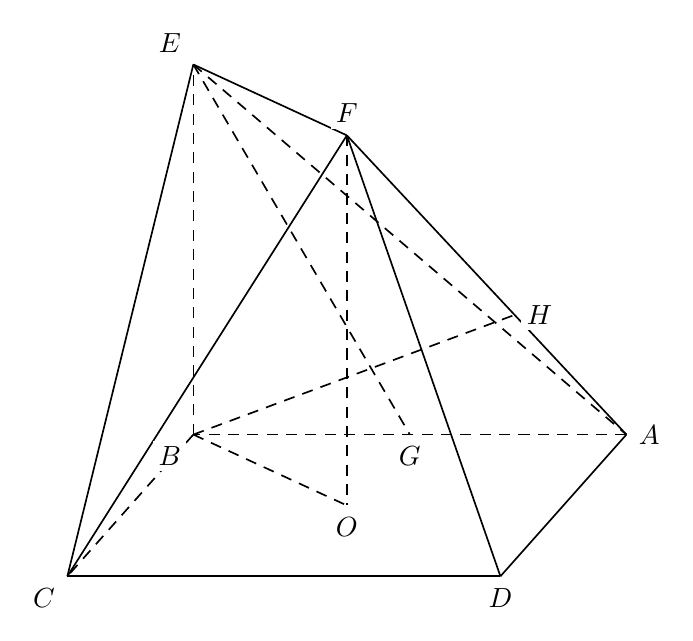
\begin{tikzpicture}[x=1cm,y=1cm,font=\normalsize]
\tikzset{solid edge/.style={solid,line width=.6pt},dashed edge/.style={dashed,dash pattern=on 4pt off 3pt,line width=.6pt},ptlabel/.style={fill=white,draw=none,inner sep=2pt,font=\normalsize}}
\coordinate (C) at (0,0);
\coordinate (D) at (5.5,0);
\coordinate (A) at (7.1000000000,1.8000000000);
\coordinate (B) at (1.6,1.8);
\coordinate (O) at (3.5500000000,0.9000000000);
\coordinate (G) at (4.3500000000,1.8000000000);
\coordinate (E) at (1.6000000000,6.5000000000);
\coordinate (F) at (3.5500000000,5.6000000000);
\coordinate (H) at (5.6800000000,3.3200000000);
\draw[solid edge] (C)--(D);
\draw[solid edge] (D)--(A);
\draw[solid edge] (C)--(E);
\draw[solid edge] (C)--(F);
\draw[solid edge] (D)--(F);
\draw[solid edge] (E)--(F);
\draw[solid edge] (F)--(H)--(A);
\draw[dashed edge] (A)--(B);
\draw[dashed edge] (B)--(C);
\draw[dashed edge] (B)--(O);
\draw[dashed edge] (B)--(E);
\draw[dashed edge] (F)--(O);
\draw[dashed edge] (E)--(G);
\draw[dashed edge] (E)--(A);
\draw[dashed edge] (B)--(H);
\node[ptlabel,anchor=north east] at ([xshift=-.8mm,yshift=-.8mm]C) {$C$};
\node[ptlabel,anchor=north] at ([yshift=-.8mm]D) {$D$};
\node[ptlabel,anchor=west] at ([xshift=.8mm]A) {$A$};
\node[ptlabel,anchor=north east] at ([xshift=-.8mm,yshift=-.8mm]B) {$B$};
\node[ptlabel,anchor=north] at ([yshift=-.8mm]O) {$O$};
\node[ptlabel,anchor=north] at ([yshift=-.8mm]G) {$G$};
\node[ptlabel,anchor=south east] at ([xshift=-.8mm,yshift=.8mm]E) {$E$};
\node[ptlabel,anchor=south] at ([yshift=.8mm]F) {$F$};
\node[ptlabel,anchor=west] at ([xshift=.8mm]H) {$H$};
\end{tikzpicture}
